Clase: 01/09/2022

\begin{teorema}[Cauchy-Gourset]
    Sea $f$ analítica en el interior y sobre el triángulo $ABC$ dado: 
    \begin{figure}[H]
        \centering 

\tikzset{every picture/.style={line width=0.75pt}} %set default line width to 0.75pt        

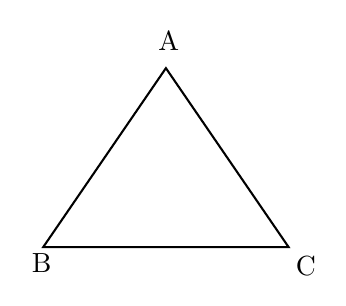
\begin{tikzpicture}[x=0.75pt,y=0.75pt,yscale=-1,xscale=1]
%uncomment if require: \path (0,300); %set diagram left start at 0, and has height of 300

%Shape: Triangle [id:dp961824107888504] 
\draw   (254.1,91) -- (313.2,177.2) -- (195,177.2) -- cycle ;

% Text Node
\draw (249,72) node [anchor=north west][inner sep=0.75pt]   [align=left] {A};
% Text Node
\draw (188,179) node [anchor=north west][inner sep=0.75pt]   [align=left] {B};
% Text Node
\draw (315.2,180.2) node [anchor=north west][inner sep=0.75pt]   [align=left] {C};


\end{tikzpicture}
    \end{figure}
    Entonces, $\int_{ABCA}f$
    \begin{dem}
        Tenemos 
        \begin{figure}[H]
            \centering
            \includegraphics[scale=0.1]{imagenes/12.1.jpeg}
        \end{figure}
        \begin{align*}
            \oint_{ABCA} f&= \int_{DAE}f+\int_{EBF}f+\int_{FCD}f\\
            &= \left[\int_{DAE}f+\int_{ED}f\right]+\left[\int_{EBF}f+\int_{FE}f\right] + \left[\int_{FCD}f+\int_{DF}f\right]\\
            &+\left[-\int_{ED}f-\int_{FE}f-\int_{DF}f\right]\\
            &= \oint_{DAED}f+\oint_{EBFE}+\oint_{FCDF}f+\left[\int_{DE}f+\int_{EF}f+\int_{FD}f\right]\\
            &= \oint_{DAED}+\oint_{EBFE}f+\oint_{FCDF}f+\oint_{DEFD}f
        \end{align*}
        Ahora bien, 

        \begin{align*}
            \left|\oint_\Delta f(z)dz\right|\leq \left|\oint_{\Delta_1} f(z)dz\right|+\left|\oint_{\Delta_2} f(z)dz\right|+\left|\oint_{\Delta_3} f(z)dz\right|+\left|\oint_{\Delta_4} f(z)dz\right|
        \end{align*}
        Sea 

        $$\left|\oint_{\Delta_1}f(x)dx\right|=\max_i\left|\oint_{\Delta_i}f(z)dz\right|$$

        $$\left|\oint_{\Delta}f(x)dz\right| \leq 4\left|\oint_{\Delta_1}f(z)dz\right|$$
        Repitiendo este proceso para $\Delta_i$, se tiene que:
        $$\left|\oint_{\Delta_1}f(x)dx\right| \leq 4\left|\oint_{\Delta_2}f(z)dz\right|$$
        $$\implies \left|\oint_{\Delta}f(x)dx\right| \leq 4^2\left|\oint_{\Delta_2}f(z)dz\right|$$
        Luego de $n$ etapas en este procesos: 
        $$\left|\oint_{\Delta}f(x)dx\right| \leq 4^n\left|\oint_{\Delta_n}f(z)dz\right|$$
        \begin{cajita}
            Nótese que $\Delta\supset \Delta_1\supset\Delta_2\supset \Delta \cdots\supset \Delta_n,\cdots $. Es decir, se tiene una sucesión anidada de triángulos.
        \end{cajita}

        Entonces, existe $z_0$ que pertenece a todos los triángulos. 
        \begin{cajita}
            \begin{lema}
                Sea $f$ analítica en una región $R$ que contiene al punto $z_0$. Entonces, 
                $$f(z)=f(z_0)+f'(z_0)(z-z_0)+\eta (z-z_0),$$
                donde $\eta\to 0$ cuando $z\to z_0$.
                \begin{dem}
                    Sea $\eta=\frac{f(z)-f(z_0)}{z-z_0}-f'(z_0)$. Como $f$ es diferenciable en $z_0$, entonces si $z\to z_0\implies \eta=0$. Por lo tanto, $f(z)=f(z_0)+f'(z_0)(z-z_0)+\eta(z-z_0)$
                \end{dem}
            \end{lema}
        \end{cajita}
        Como $f$ es analítica en $z_0$, entonces: 
        $$f(z)=f(z_0)+f'(z_0)*(z-z_0)+\eta(z-z_0),$$
        donde, se cumple que, $\forall \varepsilon >0\exists \delta>0\ni |\eta|<\varepsilon$, cuando $|z-z_0|<\frac{p}{2^n}<\delta$. Ahora 

        \begin{align*}
            \oint_{\Delta_n}f(zdz)&=\oint_{\Delta_n}f(z_0)dz+f'(z_0)\oint_{\Delta_n}(z-z_0)dz+\oint_{\Delta_n}\eta(z-z_0)dz\\
            &= \oint_{\Delta_n}\eta(z-z_0)dz
        \end{align*}
        
        \begin{cajita}
            \begin{figure}[H]
                \centering
                \includegraphics[scale=0.1]{imagenes/12.2.jpeg}
            \end{figure}
        \end{cajita}
        Entonces 

        \begin{align*}
            \left|\oint_{\Delta_n}f(zdz)\right| = \left| \oint_{\Delta_n}\eta(z-z_0)dz\right|&\leq |\eta|\cdot |z-z_0|l(\Delta_n)\\
            &< \varepsilon \frac{p}{2^n}\frac{p}{2^n}\\
            &= \frac{\varepsilon p^2}{4^n}
        \end{align*}
        $$\implies \left|\oint_\Delta f(z)dz\right|\leq 4^n \left|\oint_{\Delta_n}f(z)dz \right| <4^n \varepsilon \frac{p^2}{4^n}=\varepsilon p^2$$
        Por la arbitrariedad de $\varepsilon$, $\oint_\Delta f(z)dz =0$.
    \end{dem}
\end{teorema}

\begin{cajita}
    \begin{definicion}[R es simplemente conexo]
        Tenemos:
        \begin{enumerate}
            \item $R$ es conexo.
            \item Cada curva cerrada sobre $R$ es homotópica a un punto. 
        \end{enumerate}
        
    \end{definicion}
\end{cajita}

\begin{teorema}
    Suponga que $f$ es una función analítica sobre una región simplemente conexa. Entonces, para cualesquiera curvas $\gamma_1$ y $\gamma_2$ que unen $z_0$ con $z$, en $A$, se tiene que: 
    $$\int_{\gamma_1}f=\int_{\gamma_2}f$$
    \begin{dem}
        Tenemos: 
        \begin{figure}[H]
            \centering
            \includegraphics[scale=0.1]{imagenes/12.3.jpeg}
        \end{figure}
        Sea $\gamma =\gamma_1-\gamma_2$.
        $$\implies \int_\gamma f = \int_{\gamma_1-\gamma_2}f=\int_{\gamma_1}f-\int_{\gamma_2}f=0.$$
    \end{dem}
\end{teorema}


